\chapter{Problema inverso} \label{cha:pi}

\section{Definindo o problema inverso} \label{sec:pi-def}
Resolver um problema inverso é em sua essencial descobrir qual a entrada atual para um problema para o qual só se conhece o modelo direto no processo de resolução e as suas saídas, ou seja, não se utiliza um modelo, seja caixa preta ou caixa branca, que reproduza o comportamento inverso do sistema analisado naquele momento \cite{ljung1999system}. É a partir de um processo de otimização das entradas, e não de qualquer coeficiente presente no modelo, se faz a busca da entrada que produza a saída conhecida.

A \autoref{fig:pi-exemplo} evidência a estrutura do problema inverso, no qual uma entrada inicial é proposta como solução para o algoritmo de otimização. A partir disso, o algoritmo começa a explorar o espaço das entradas, até encontrar uma que reduza o erro entre a saída do modelo e a saída esperada a ponto da condição de busca terminar. Essa condição em geral é uma combinação do número máximo de iterações, do valor do erro e da estabilidade do valor do erro.

\imagem{Modelo de resolução do problema inverso}{
\resizebox{0.8\textwidth}{!}{
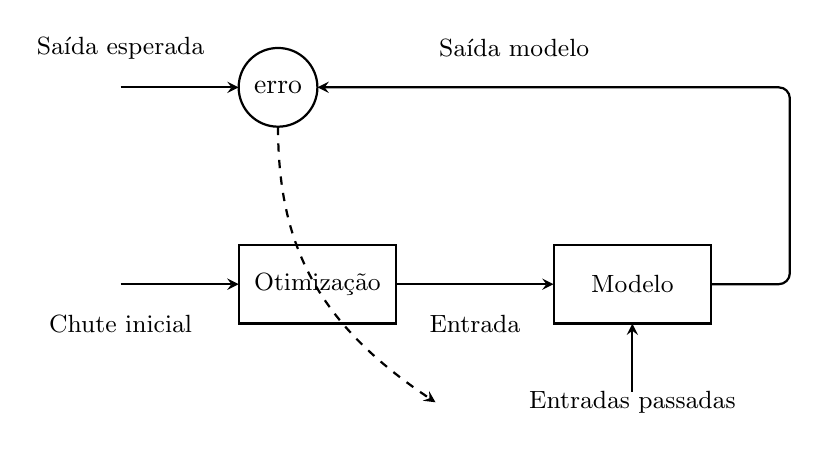
\begin{tikzpicture}[shorten <=0.01pt,shorten >=0.01pt,>=stealth,thick,->]
\draw  (1,2) ellipse (0.5 and 0.5) node (v1) {erro};
\draw  (0.5,0) rectangle node {\small Otimização} (2.5,-1);
\draw  (4.5,0) rectangle node {\small Modelo} (6.5,-1);
\draw  (2.5,-0.5) -- (4.5,-0.5);
\draw[dashed] (1,1.5) .. controls (1,0) and (1.5,-1) .. (3,-2);
\draw (-1,-0.5) -- (0.5,-0.5);
\draw[rounded corners=4pt] (6.5,-0.5) -- (7.5,-0.5) -- (7.5,2) -- (1.5,2);
\node at (-1,-1) {\small Chute inicial};
\node at (3.5,-1) {\small Entrada};
\node at (4,2.5) {\small Saída modelo};
\draw  (-1,2) -- (0.5,2);
\node at (-1,2.5) {\small Saída esperada};
\node (v2) at (5.5,-2) {};
\node at (v2) {\small Entradas passadas};
\draw  (v2) edge (5.5,-1);
\end{tikzpicture}
}
\label{fig:pi-exemplo}
}{O autor}{fig:pi-exemplo}{}{Modelo de resolução do problema inverso, possuindo como parâmetros um chute inicial, uma saída esperada e as entradas passadas com o objetivo de encontrar uma entrada que minimize o erro entre a saida esperada e a saída do modelo.}

O problema inverso é utilizado em diversas áreas, em especial na área de computação de imagens, no qual pode ser utilizado para a reconstrução de imagens na área médica \cite{mccann2016fast}, no aumento da resolução de imagens de microscópios \cite{kellman2019data}, entre outros usos \cite{9084378}.

\section{Problemas bem-postos e mal-postos} \label{sec:pi-posto}
Uma das maneiras de se classificar um problema é se este é bem-posto ou se é mal-posto, sendo problemas bem-postos normalmente estáveis para as soluções numéricas, enquanto problemas mal-postos possuem uma maior complexidade para a sua resolução. Conforme os critérios de Hadamard \cite{hadamard1902problemes}, existem três condições para que um problema seja considerado bem-posto:
\begin{itemize}
  \item Uma solução exista
  \item Está solução seja única
  \item O comportamento desta solução seja contínuo
\end{itemize}

Visto que o problema inverso consiste em encontrar as entradas de um modelo conhecendo-se as suas saídas e sabendo-se que o problema inverso é geralmente avaliado para funções não monotônicas, é fácil entender que o problema inverso em geral é um problema mal-posto.
No caso em específico do PA isto é uma certeza, pois não existe uma solução única para todas as saídas em uma função não monotônica, portanto o problema inverso do PA é mal-posto. Logo, métodos numéricos aplicados na resolução do problema inverso possuem uma possibilidade de convergir para um valor incorreto ou de não conseguirem convergir. O processo utilizado para a modelagem do PA também é responsável por outras dificuldades que tornam mais complexa a análise e o entendimento dos resultados obtidos.

\section{Aplicação do problema inverso para a análise comportamental} \label{sec:pi-app}
Para se analisar o comportamento do modelo direto do amplificador de potência com a utilização do problema inverso não é necessária nenhuma modificação na estrutura presente na \autoref{fig:pi-exemplo}. No entanto, as entradas passadas, em razão do modelo possuir memória, devem ser passadas como parâmetros adicionais ao modelo.